
\gls{idealFluid}运动的基本方程

\gls{idealFluid}应力张量$T_{ij}=-p\delta_{ij}$,因此动量方程\eqref{eq:52Momen}式化为:
\begin{equation}\label{eq:62EulerEq}
 \frac{\partial \v{v}}{\partial t}+\v{v}\cdot\nabla\v{v}=\v{f}-\frac{1}{\rho}\nabla\cdot p
\end{equation}
\eqref{eq:62EulerEq}式即欧拉方程,
相应的\eqref{eq:52Energy}化为
\begin{equation}\label{eq:62IdealEnergy}
 \frac{D(e+\frac{1}{2}|\v{v}|^2)}{Dt}=
 \v{f}\cdot\v{v}-\frac{1}{\rho}\nabla\cdot(p\v{v})+(\dot{q}+q_R) 
\end{equation}

综合连续性方程\eqref{eq:52Conti}式,\eqref{eq:62EulerEq},\eqref{eq:52Energy}
共5个方程,但未知数有$\v{v},e,p,\rho\,$ 6个,因此需补充热力学方程才能使方程组封闭。

实际上,我们可以通过动量方程\eqref{eq:62EulerEq}式得到动能的变化率:
\begin{equation}\label{eq:62KinematicEneryChangeRate}
\frac{D}{D t}(\frac{1}{2}|\v{v}|^2)=\v{f}\cdot \v{v}-\frac{1}{\rho}\v{v}\cdot\nabla p
\end{equation}
将\eqref{eq:62IdealEnergy}式与\eqref{eq:62KinematicEneryChangeRate}作差得:
\begin{align}
\frac{De}{Dt}= & -\frac{p}{\rho} \nabla \cdot \v{v} + \dot{q}+q_R ,\text{by }\eqref{eq:52ContiMaterial}\nonumber\\
=& \frac{p}{\rho^2}\frac{D\rho}{Dt} + \dot{q}+q_R \nonumber\\
=& -p\frac{D}{Dt}\left(\frac{1}{\rho}\right) + \dot{q}+q_R\label{eq:62DeDt1}
\end{align}
定义$i=e+\frac{p}{\rho}$为气体的焓,则可以得到
\begin{equation}
\frac{D i}{D t}=\dot{q}+q_R + \frac{1}{\rho} \frac{D p }{D t}
\end{equation}
对于绝热状态下的理想常比热完全气体,我们有
\begin{align}
\frac{D e}{D t}=& C_V \frac{D T}{D t},e=C_V T\nonumber\\
=& \frac{C_V}{R} \frac{D}{D t}\left(\frac{p}{\rho}\right),p=\rho RT\nonumber\\
=& \frac{1}{\gamma -1} \frac{D}{D t}\left(\frac{p}{\rho}\right),C_P-C_V=R,\frac{C_P}{C_V}=\gamma \label{eq:62DeDt2}
\end{align}
将\eqref{eq:62DeDt1}式去掉产热项,与\eqref{eq:62DeDt2}式结合可以得到
\begin{equation}\label{eq:62prho}
\frac{D}{D t}\left(\frac{p}{\rho^{\gamma}}\right)=0
\end{equation}
\eqref{eq:62prho}式即为对于气体补充的$\rho$和$p$的关系的热力学方程。

对于匀质不可压缩的液体,补充$\nabla \cdot \v{v}=0$的方程,此时\eqref{eq:52Conti}式恒成立,动力学方程与热力学方程解耦,
因此我们可以联立求解:
\begin{align}\notag
\nabla \cdot \v{v}=&0\\
 \frac{\partial \v{v}}{\partial t}+\v{v}\cdot\nabla\v{v} =&\v{f}-\frac{1}{\rho}\nabla  p \label{eq:62IdealFluid}
\end{align}
得到$\v{v},p$再代入能量方程求其他参量。

下面考虑\gls{idealFluid}动力学偏微分方程的边界条件。一般的,对于不可穿透的壁面,流体的法向速度与壁面运动的法向速度相等,即满足:
\begin{equation}
(\v{v}_L\cdot \v{n})_{\Sigma}=(\v{v}_B\cdot \v{n})_{\Sigma}
\end{equation}
若$\Sigma$有曲面方程$F(x,y,z,t)=0$,则流体边界速度满足
\begin{equation}\label{eq:62BCSur}
\frac{\partial F}{\partial t} + \v{v_L} \cdot \nabla F=0
\end{equation}
此即\textbf{不可穿透条件}的一种提法;此外,我们还有无穷远条件等。

比如考虑一半轴长分别为$a,b,c$的实心椭球,以速度$U\v{i}$在流体中运动,则在椭球面上流体的边界条件可根据椭球面方程求出。
在固结在椭球中心的运动参考系中$(O'x'y'z')$中,椭球面方程为
\begin{equation}
F':\frac{x'^2}{a^2}+\frac{y'^2}{b^2}+\frac{z'^2}{c^2}-1=0
\end{equation}
$F'$不随时间变化,由\eqref{eq:62BCSur}式得到在$(O'x'y'z')$中速度的边界条件为
\begin{equation}
\frac{u'x'}{a^2}+\frac{v'y'}{b^2}+\frac{w'z'}{c^2}=0
\end{equation}
若考虑静止参考系$(Oxyz)$,则
\begin{equation}
F:\frac{(x-Ut)^2}{a^2}+\frac{y^2}{b^2}+\frac{z^2}{c^2}-1=0
\end{equation}
$F$随时间变化,可得在$(Oxyz)$中速度的边界条件为
\begin{equation}
\frac{-U(x-Ut)}{a^2}+\frac{u(x-Ut)}{a^2}+\frac{vy}{b^2}+\frac{wz}{c^2}=0
\end{equation}

下面应用\gls{idealFluid}动力学方程组\eqref{eq:62IdealFluid}式求解一个球对称问题:考虑无限大的液体中有一匀质圆球均匀地向外膨胀,半径
$R$随时间变化规律为$R=R_b(t)$,已知初始时刻$t=0$时液体静止,求解$t$时刻液体压强的分布。

首先由球对称性可以得到$\v{v}=v_r\v{e_r}$
对于球坐标,基矢量随坐标变量的变化规律为\cite{Del}:
\begin{align}
\frac{\partial \v{e_r}}{\partial \theta}=&\v{e_{\theta}},\,\,  \frac{\partial \v{e_r}}{\partial \varphi}=\v{e_{\varphi}}\sin\theta\\
\frac{\partial \v{e_{\theta}}}{\partial \theta}=&-\v{e_r},\,\,  \frac{\partial \v{e_{\theta}}}{\partial \varphi}=\v{e_{\varphi}}\cos\theta\\
\frac{\partial \v{e_{\varphi}}}{\partial \varphi}=&-(\v{e_r}\sin\theta+\v{e_{\theta}}\cos\theta)
\end{align}

球坐标系下的梯度算子表示为:
\begin{equation}
\nabla = \frac{\partial }{\partial r} \v{e_r} + \frac{1}{r} \frac{\partial}{\partial \theta} \v{e_{\theta}}+
\frac{1}{r\sin\theta}
\frac{\partial }{\partial \varphi}\v{e_{\varphi}}
\end{equation}

因此球坐标系下对于矢量$\v{v}=v_r\v{e_r}+v_{\theta}\v{e_{\theta}}+v_{\varphi}\v{e_{\varphi}}$的散度为:
\begin{align*}
&(\frac{\partial }{\partial r} \v{e_r} + \frac{1}{r} \frac{\partial}{\partial \theta} \v{e_{\theta}}+\frac{1}{r\sin\theta}
\frac{\partial }{\partial \varphi}\v{e_{\varphi}})\cdot (v_r\v{e_r}+v_{\theta}\v{e_{\theta}}+v_{\varphi}\v{e_{\varphi}}) =\\
&\frac{\partial v_r}{\partial r}+\frac{1}{r}\frac{\partial v_{\theta}}{\partial \theta}+\frac{1}{r\sin\theta}
\frac{\partial v_{\varphi}}{\partial \varphi} +\frac{v_r}{r}\frac{\partial \v{e_r}}{\partial \theta}\cdot \v{e_{\theta}}+
(v_r\frac{\partial \v{e_r}}{\partial \varphi}+v_{\theta}\frac{\partial \v{e_{\theta}}}{\partial \varphi}+
v_{\varphi}\frac{\partial \v{e_{\varphi}}}{\partial \varphi})\cdot \frac{\v{e_{\varphi}}}{r \sin\theta}\\
=&\frac{\partial v_r}{\partial r}+\frac{1}{r}\frac{\partial v_{\theta}}{\partial \theta}+\frac{1}{r\sin\theta}
\frac{\partial v_{\varphi}}{\partial \varphi} +\frac{v_r}{r}+
(v_r\sin\theta+v_{\theta}\cos\theta)\frac{1}{r \sin\theta}\\
=&\frac{\partial v_r}{\partial r}+\frac{1}{r}\frac{\partial v_{\theta}}{\partial \theta}+\frac{1}{r\sin\theta}
\frac{\partial v_{\varphi}}{\partial \varphi} +\frac{2v_r}{r}+\frac{v_{\theta}\cos\theta}{r \sin\theta}
\end{align*}
所以
\begin{equation}
\nabla \cdot \v{v}=\frac{1}{r^2}\frac{\partial (r^2 v_r)}{\partial r}+
\frac{1}{r\sin\theta}\frac{\partial (v_{\theta}\sin\theta)}{\partial \theta}+
\frac{1}{r\sin\theta}\frac{\partial v_{\varphi}}{\partial \varphi} 
\end{equation}
由上式以及\eqref{eq:62IdealFluid}式中的不可压缩方程,我们得到
\begin{equation}
\frac{\partial (r^2 v_r)}{\partial r}=0
\end{equation}
结合$r=R$时$v_r=\dot{R}_b(t)$于是得到
\begin{equation}\label{eq:62vrResult}
v_r=\frac{R_b(t)^2}{r^2}\dot{R}_b(t)
\end{equation}
对于\eqref{eq:62IdealFluid}式中的动量方程,$\v{v}\cdot \nabla =v_r\frac{\partial}{\partial r}$,因此动量方程化为
\begin{equation}\label{eq:62pResult}
\frac{\partial v_r}{\partial t}+v_r \frac{\partial v_r}{\partial r}=-\frac{1}{\rho}\frac{\partial p}{\partial r}
\end{equation}
代入\eqref{eq:62vrResult}式到\eqref{eq:62pResult}式中,得到
\begin{equation}
p=p_{\infty}+\frac{\rho R_b}{2r^4}((4r^3-R_b^3)\dot{R}_b^2+2r^3R_b\ddot{R}_b)
\end{equation}
令$r=R_b$得到球外表面压力分布为
\begin{equation}
p_{ext}=p_{\infty}+\rho(R_b\dot{R}_b^2+\frac{3}{2}\dot{R}_b^2)
\end{equation}
对液体表面薄层受力分析可得到内外压关系(假设圆球内是压强分布均匀的气体)为
\begin{equation}
p_{int}=p_{ext}+\frac{2\gamma}{R}
\end{equation}
其中$\gamma$是液体的表面张力系数,如已知$p_{int}$,解上式ODE可得$R=R(t)$即界面随时间变化规律。

\gls{idealFluid}在势力场中运动的主要性质:
\newglossaryentry{KelvinTheorem}
{
  name=Kelvin 定理,
  description=若下列4个条件同时成立,则速度场沿流线的环量积分不变:
\begin{itemize}
\item 流场连续
\item 流体是\gls{barotropic}
\item 流体是\gls{idealFluid}
\item 质量力有势
\end{itemize}
}
\gls{KelvinTheorem},也称环量不变定理,指出\glsdesc{KelvinTheorem}

\gls{KelvinTheorem}的数学表述为:
\begin{equation}\label{eq:62KelvinMath}
\frac{D}{Dt} \left(\oint_{l}\v{v}\cdot d\v{x}\right) =0
\end{equation}

\begin{figure}[!ht]
 \centering
 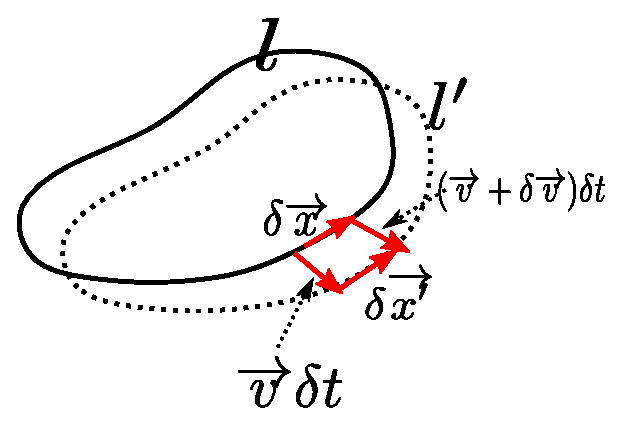
\includegraphics[width=5cm]{KelvinTheorem.eps}
 \caption{Kelvin 定理推导图示}\label{fig:62Kelvin}
\end{figure}
推导\eqref{eq:62KelvinMath}式可按如下步骤:
\begin{align*}
\frac{D}{Dt} \left(\oint_{l}\v{v}\cdot d\v{x}\right)= &  \oint_{l}\frac{D}{Dt}(\v{v}\cdot d\v{x})\\
=& \oint_{l}\frac{D \v{v}}{Dt} \cdot d\v{x} +\oint_l \v{v}\cdot \frac{D(d\v{x})}{Dt}\\
=& I_1+I_2
\end{align*}
对于$I_2$,由图\ref{fig:62Kelvin},假设$\delta t$时间流线$l$变到了$l'$,流线上的微元质量体$\delta \v{x}$变到
了$\delta \v{x'}$,则有矢量关系
$\delta \v{x}+(\v{v}+\delta \v{v})\delta t = \v{v}\delta t+\delta \v{x'}$
成立,即$\delta \v{x'}-\delta \v{x}=\delta \v{v} \delta t$,从而$d\v{x}$的随体导数为$ d\v{v}$,
注意到$\v{v}\cdot d\v{v}=d(\frac{1}{2}|\v{v}|^2)$,而动量的环量积分为零。因此$I_2=0$。

对于$I_1$,由\eqref{eq:62IdealFluid}式中的动量方程$\frac{D \v{v}}{Dt}=\v{f}-\frac{\nabla p}{\rho}$,
根据假设流体是\gls{barotropic},因此由\eqref{eq:61barotropicPotential}式得存在压力函数$\mathbb{P}$
使得$\frac{\nabla p}{\rho}=\nabla \mathbb{P}$,又因为质量力有势,所以又存在势力场$\Pi$使得$\v{f}=-\nabla \Pi$,
于是
\begin{align*}
I_1 = & \oint_{l}\frac{D \v{v}}{Dt} \cdot d\v{x}\\
= & -\oint_{l}\nabla(\Pi + \mathbb{P})\cdot d\v{x}\\
= & 0
\end{align*}
因此,\eqref{eq:62KelvinMath}式成立。

由\gls{KelvinTheorem}可直接导出Lagrange 定理,也称涡量不生不灭定理,即在\gls{KelvinTheorem}成立的条件下,流场若一开始有旋则始终有旋,一开始无旋则
始终无旋。只需利用Stokes公式即可说明。

由Lagrange定理的逆否可以得到旋涡产生或消失的条件是\gls{KelvinTheorem}的四个条件至少有一个不能满足。


